\chapter{Background to Classical Planning}\label{ch:background}
\chapterquote{[Binary Decision Diagrams are] one of the only really fundamental data structures that came out in the last twenty-five years.}{Donald Knuth (2008)}

In AI planning, the objective is to automatically find a solution (a plan) to a given problem (a planning task).
In this chapter, we formally define classical planning and discuss the concepts of complexity, compilability and expressive power in this context.
Finally, symbolic search for classical planning is presented and different types of decision diagrams are introduced.

\section{Formalism}
In this thesis, we consider classical planning domains and tasks that are characterized by the \name{sas}$^+$ formalism \autocite{backstrom-nebel-compint1995}.

\begin{definition}[Planning Domain]
  \label{def:planning-domain}
  A \emph{planning domain} is a tuple $\domain = \domaintuple$. $\vars$ is a finite set of state variables, each associated with a finite domain $\vardomain{}_v = \{0, \dots, |\vardomain{}_v| - 1\}$. A \emph{fact} is a pair $(v, d)$, where $v \in \vars$ and $d \in \vardomain_v$. For binary variables we also write $v$ for $(v,1)$ and $\lnot v$ for $(v,0)$. A \emph{partial state} or \emph{partial variable assignment} $s$ over $\vars$ is a function on some subset of $\vars$ such that $s(v) \in \vardomain{}_v$, wherever $s(v)$ is defined. If $s$ assigns a value to each variable $v \in \vars$, $s$ is called a \emph{state}. With $\states$ we refer to the set of all possible states defined over $\vars$. $\operators$ is a finite set of \emph{operators/actions}, where each operator is a pair $o = \langle \pre_o, \eff_o \rangle$ of partial variable assignments, called \emph{preconditions} and \emph{effects}. An operator $o \in \operators$ is applicable in a state $s$ iff $\pre_o$ is satisfied in $s$, i.e., $\pre_o \subseteq s$. Applying operator $o$ to state $s$ yields the state $s[o]=s'$, where $s'(v) = \eff_o(v)$ for all variables $v \in \vars$ for which $\eff_o$ is defined and $s'(v) = s(v)$ otherwise. Finally, $\constcostfun: \operators \to \mathbb{N}_0$ is the \emph{cost function} of $\domain$. The size of $\domain$ is $\size{\domain} = \sum_{v \in \vars}|\vardomain{}_v| + \sum_{o \in \operators}(|\pre_o| + |\eff_o|) + \size{\constcostfun}$, where $\size{\constcostfun}$ is bounded by $|\operators| \cdot \lceil \log_2 N \rceil$, where $N$ is the highest action cost value.
\end{definition}

Planning domains together with initial states and goal descriptions form planning tasks.

\begin{definition}[Planning Task]
  \label{def:planning-task}
  A \emph{planning task} is a tuple $\task = \langle \domain, \init, \goal, \limit \rangle$ consisting of a \emph{planning domain}, an \emph{initial state} $\init \in \states$, a partial variable assignment $\goal$ (\emph{goal condition}), which defines all possible goal states $\goalstates \subseteq \states$, and a \emph{cost bound} $\limit \in \mathbb{N}_0 \cup \{ \infty \}$. For simplicity, we also write $\langle \vars, \operators, \constcostfun, \init, \goal \rangle$ for a planning task with domain $\domain = \domaintuple$ and $\limit = \infty$.
  The \emph{size} of $\task$ is $\size{\task} = \size{\domain} + |\goal| + |\init| + \size{\limit}$, where $\size{\limit} = \lceil \log_2 B \rceil$ is the binary encoding size of the cost bound.
\end{definition}

A planning task is often defined without a cost bound $\limit$, which is equivalent to setting the cost bound to infinity (or a sufficient upper bound). However, we use planning tasks with cost bounds to perform complexity and compilability analyses in this dissertation.

The objective of classical planning is to determine plans, which are sequences of applicable actions leading from the initial state to a goal state, respecting the given cost bound $\limit$.

\begin{definition}[Plan]
  \label{def:plan}
  A \emph{plan} $\plan = \langle o_0, \dots, o_{n-1} \rangle$ for planning task
  $\task$ is a sequence of applicable operators that generates a sequence of
  states $s_0, \dots, s_n$, where  $s_0 = \init$, $s_n \in \goalstates$ is a goal state, $s_{i+1} = s_i[o_i]$ for all $i = 0, \dots, n-1$, and the \emph{cost} of $\pi$ is less than or equal to the cost bound $\limit$, i.e., $\cost(\plan) = \sum_{i=0}^{{n-1}} \constcostfun(o_i) \leq \limit$. Plan $\pi$ is \emph{optimal} if
  there is no cheaper plan. We call $\size{\plan} = n$ the \emph{length} or \emph{size} of $\plan$. With $P_\task$ we refer to the (possibly infinite) \emph{set of all plans} for a planning task $\task$.
\end{definition}

The search for an optimal plan, i.e., a plan with the lowest cost, is called cost-optimal planning, or optimal planning for short, and is the focus of this thesis. 
\Cref{ex:rover} describes a classical planning domain and task of a Mars rover, which we will use in this work to motivate and explain expressive features that extend the classical planning formalism.

\begin{example}\label{ex:rover}
  Consider a Mars rover like Perseverance\footnote{\label{note1}\url{https://mars.nasa.gov/mars2020/mission/overview/} (Accessed: 2021-10-12)} equipped with a drone like Ingenuity\footref{note1}, which are designed to perform autonomous tasks. 
  Such a scenario is illustrated in \Cref{fig:mars_example}. 
  The dynamics of this example, i.e., the domain, are as follows.

  The rover can navigate between adjacent cells if they are free (impassable cells are highlighted in red). Navigating the rover between cells has no cost, i.e., a cost of $0$. The drone can launch and land on the rover if both are in the same location. Launching and landing each has a cost of $5$. In addition, the drone can take an image at its current position at a cost of $2$ and fly between any two cells, ignoring the impassability of cells to the rover. The cost of flying from one cell $\textit{from} = (x,y)$ to another cell $\textit{to} = (x',y')$ is the Manhattan distance between these two cells, i.e., $|x-x'|+|y-y'|$.

  In this particular planning task, the rover along with the drone is initially located at (7,3), the actual landing site of Perseverance. The goal is to take pictures at (6,1) and (10,1) and travel with the drone equipped to (0,5), a location known as ``Three Forks'' from which new missions can be commenced.  The cost bound for this task is infinite.

  An optimal plan for this task is $\pi^\rover{} = \langle$\navigate{7}{2},  \navigate{7}{1}, \startDrone{7}{1}, \fly{7}{1}{6}{1}, \takeImg{6}{1}, \fly{6}{1}{10}{1}, \takeImg{10}{1}, \fly{10}{1}{7}{1}, \landDrone{7}{1}, \navigate{7}{2}, \navigate{7}{3}, \dots, \navigate{0}{5}$\rangle$ with a cost of $\cost(\pi^\rover{}) = 5 + 5 + 2 \cdot 2 + 8 = 24$, since navigating the rover costs $0$, the drone launches and lands once with a cost of $5$ each, takes images twice with a cost of $2$ each, and flies a total distance of $8$ cells.

  % Formally, the Rover planning domain $\roverdomain = \langle \rovervars, \roveroperators, \roverconstcostfun \rangle$ and rover task $\rovertask = \langle \roverdomain, \roverinit, \rovergoal, \roverlimit \rangle$ are definied as follows.

  % \begin{compactitem}
  %   \item $\rovervars = \{\textit{rover-at-x}, \textit{rover-at-y}, \textit{drone-at-x}, \textit{drone-at-y}, \textit{drone-on-rover}\} \\
  %           \phantom{\rovervars} \cup \{\textit{adjacent-}x_1\textit{-}x_2 ~|~ x_1, x_2 \in \{0,\dots,10\} \} \\
  %           \phantom{\rovervars} \cup \{\textit{adjacent-}y_1\textit{-}y_2 ~|~ y_1, y_2 \in \{0,\dots,8\} \} \\
  %           \phantom{\rovervars} \cup \{\textit{free-}x\textit{-}y, \textit{taken-image-}x\textit{-}y ~|~ x \in \{0,\dots,10 \}, y \in \{0,\dots,8\} \}
  %         $
  %   \item $\vardomain_{\textit{rover-at-x}} = \vardomain_{\textit{drone-at-x}} = \{0,\dots,10\}$
  %   \item $\vardomain_{\textit{rover-at-y}} = \vardomain_{\textit{drone-at-y}} = \{0,\dots,8\}$
  %   \item $\vardomain_{v} = \{0,1\} \text{   if } v \in \rovervars \setminus \{\textit{rover-at-x}, \textit{rover-at-y}, \textit{drone-at-x}, \textit{drone-at-y}\}$
  %   \item $\roveroperators = \{\textit{move-}x_1y_1\textit{-}x_2y_2 ~|~ x_1,x_2 \in \{0,\dots,10\} \land y_1,y_2 \in \{0,\dots,8\}\}$
  % \end{compactitem}
\end{example}

\begin{figure}
  \begin{center}
    \pgfdeclareshape{quadcopter side}{
    \inheritsavedanchors[from=coordinate]
    \inheritanchor[from=coordinate]{center}
    \backgroundpath{
        \begin{pgfscope}
            \pgftransformshift{\centerpoint}
            \pgfmathdivide{\pgfkeysvalueof{/pgf/minimum width}}{1pt}
            \pgftransformscale{\pgfmathresult}
            \pgfpathmoveto{\pgfpoint{-0.3}{-0.02}}
            \pgfpathlineto{\pgfpoint{0.3}{-0.02}}
            \pgfpathlineto{\pgfpoint{0.3}{0.02}}
            \pgfpathlineto{\pgfpoint{-0.3}{0.02}}
            \pgfpathclose
            \pgfpathmoveto{\pgfpoint{0.25}{0.02}}
            \pgfpathlineto{\pgfpoint{0.25}{0.15}}
            \pgfpathclose
            \pgfpathmoveto{\pgfpoint{-0.25}{0.02}}
            \pgfpathlineto{\pgfpoint{-0.25}{0.15}}
            \pgfpathclose
            \pgfpathmoveto{\pgfpoint{-0.35}{0.15}}
            \pgfpathlineto{\pgfpoint{-0.15}{0.15}}
            \pgfpathclose
            \pgfpathmoveto{\pgfpoint{0.15}{0.15}}
            \pgfpathlineto{\pgfpoint{0.35}{0.15}}
            \pgfpathclose
            \pgfpathmoveto{\pgfpoint{0}{0.02}}
            \pgfpathlineto{\pgfpoint{0}{0.1}}
            \pgfpathclose
            \pgfpathmoveto{\pgfpoint{-0.1}{0.1}}
            \pgfpathlineto{\pgfpoint{0.1}{0.1}}
            \pgfpathclose
        \end{pgfscope}}}
\scalebox{0.89}{
    \begin{tikzpicture}
        \begin{scope}
            \clip(0,0) rectangle (11,8);
            \node[inner sep=0pt,anchor=south west] at (0.0,0)
            {\includegraphics[width=11.30cm]{pictures/jezero_mars.png}};
        \end{scope}
        \tkzInit[xmax=11,ymax=8,xmin=0,ymin=0]
        \tkzGrid[color=lightgray]
        %\tkzAxeXY
        \tkzDrawY[label=$y$]
        \foreach \y in {0,...,7} {% 
                \tkzLabelPoint[left=1pt](0,\y.5){$\y$}}
        \tkzDrawX[label=$x$]
        \foreach \x in {0,...,10} {% 
                \tkzLabelPoint[below=1pt](\x.5,0){$\x$}}

        \def\alphavalue{0.2}
        \draw[fill=red,opacity=\alphavalue] (3,0) rectangle ++(1,1);
        \draw[fill=red,opacity=\alphavalue] (4,0) rectangle ++(1,1);
        \draw[fill=red,opacity=\alphavalue] (8,0) rectangle ++(1,1);
        \draw[fill=red,opacity=\alphavalue] (9,0) rectangle ++(1,1);

        \draw[fill=red,opacity=\alphavalue] (3,1) rectangle ++(1,1);
        \draw[fill=red,opacity=\alphavalue] (4,1) rectangle ++(1,1);
        \draw[fill=red,opacity=\alphavalue] (6,1) rectangle ++(1,1);
        \draw[fill=red,opacity=\alphavalue] (8,1) rectangle ++(1,1);
        \draw[fill=red,opacity=\alphavalue] (9,1) rectangle ++(1,1);

        \draw[fill=red,opacity=\alphavalue] (0,2) rectangle ++(1,1);
        \draw[fill=red,opacity=\alphavalue] (2,2) rectangle ++(1,1);
        \draw[fill=red,opacity=\alphavalue] (3,2) rectangle ++(1,1);
        \draw[fill=red,opacity=\alphavalue] (4,2) rectangle ++(1,1);
        \draw[fill=red,opacity=\alphavalue] (5,2) rectangle ++(1,1);
        \draw[fill=red,opacity=\alphavalue] (6,2) rectangle ++(1,1);
        \draw[fill=red,opacity=\alphavalue] (8,2) rectangle ++(1,1);
        \draw[fill=red,opacity=\alphavalue] (9,2) rectangle ++(1,1);
        \draw[fill=red,opacity=\alphavalue] (10,2) rectangle ++(1,1);

        \draw[fill=red,opacity=\alphavalue] (0,3) rectangle ++(1,1);
        \draw[fill=red,opacity=\alphavalue] (2,3) rectangle ++(1,1);
        \draw[fill=red,opacity=\alphavalue] (3,3) rectangle ++(1,1);
        \draw[fill=red,opacity=\alphavalue] (4,3) rectangle ++(1,1);
        \draw[fill=red,opacity=\alphavalue] (5,3) rectangle ++(1,1);
        \draw[fill=red,opacity=\alphavalue] (6,3) rectangle ++(1,1);
        \draw[fill=red,opacity=\alphavalue] (8,3) rectangle ++(1,1);
        \draw[fill=red,opacity=\alphavalue] (9,3) rectangle ++(1,1);
        \draw[fill=red,opacity=\alphavalue] (10,3) rectangle ++(1,1);

        \draw[fill=red,opacity=\alphavalue] (2,4) rectangle ++(1,1);
        \draw[fill=red,opacity=\alphavalue] (3,4) rectangle ++(1,1);
        \draw[fill=red,opacity=\alphavalue] (4,4) rectangle ++(1,1);
        \draw[fill=red,opacity=\alphavalue] (5,4) rectangle ++(1,1);
        \draw[fill=red,opacity=\alphavalue] (6,4) rectangle ++(1,1);

        \draw[fill=red,opacity=\alphavalue] (5,5) rectangle ++(1,1);
        \draw[fill=red,opacity=\alphavalue] (6,5) rectangle ++(1,1);
        \draw[fill=red,opacity=\alphavalue] (7,5) rectangle ++(1,1);
        \draw[fill=red,opacity=\alphavalue] (8,5) rectangle ++(1,1);
        \draw[fill=red,opacity=\alphavalue] (9,5) rectangle ++(1,1);

        \draw[fill=red,opacity=\alphavalue] (0,6) rectangle ++(1,1);
        \draw[fill=red,opacity=\alphavalue] (1,6) rectangle ++(1,1);
        \draw[fill=red,opacity=\alphavalue] (2,6) rectangle ++(1,1);
        \draw[fill=red,opacity=\alphavalue] (6,6) rectangle ++(1,1);
        \draw[fill=red,opacity=\alphavalue] (7,6) rectangle ++(1,1);
        \draw[fill=red,opacity=\alphavalue] (8,6) rectangle ++(1,1);

        \draw[fill=red,opacity=\alphavalue] (0,7) rectangle ++(1,1);
        \draw[fill=red,opacity=\alphavalue] (1,7) rectangle ++(1,1);
        \draw[fill=red,opacity=\alphavalue] (2,7) rectangle ++(1,1);
        \draw[fill=red,opacity=\alphavalue] (3,7) rectangle ++(1,1);

        \node[] at (6.5,1.5) {\Large \color{white}{\faCamera}};
        \node[] at (10.5,1.5) {\Large \color{white}{\faCamera}};
        \node[] at (0.5,5.5) {\rotatebox{180}{\Large \color{white}{\faSignOut}}};
        \node[quadcopter side,fill=white,draw=white,minimum width=1.2cm] at (7.5,3.5) {};

        \begin{scope}[xshift=7.5cm,yshift=3.3cm]
            \draw[white,line width=0.075cm] (-0.4,0) -- (0.4, 0);
            \node[regular polygon,regular polygon sides=7,draw,white,scale=0.375,line width=0.035cm] at (-0.3,-0.175) {};
            \node[regular polygon,regular polygon sides=7,draw,white,scale=0.375,line width=0.035cm] at (0.0,-0.175) {};
            \node[regular polygon,regular polygon sides=7,draw,white,scale=0.375,line width=0.035cm] at (0.3,-0.175) {};
        \end{scope}

        %\tkzDefPoint(1,1){E_{1, 1}}
        %\tkzDefPoint(2,3){E_{2, 3}}
        %\tkzDrawPoints(E_{1, 1}, E_{2, 3})
        %\tkzLabelPoints(E_{1, 1}, E_{2, 3})
        %\tkzText[above](0,6.75){A Sample Grid}
    \end{tikzpicture}
}
  \end{center}
  \caption[Visualization of the Mars rover planning task (running example).]{Visualization of the Mars rover planning task used as a running example. The original image is from NASA/JPL-Caltech/University of Arizona\protect\footnotemark{} and shows the Jezero crater, where the green dot indicates the actual landing site of the Perseverance rover.
  Rover, drone, grid lines, red coloring (impassable cells for the rover), camera (goal: take pictures), and arrow (goal: cell to which the rover should travel with the drone) are added.}
  \label{fig:mars_example}
\end{figure}
\footnotetext{\url{https://mars.nasa.gov/resources/25621/perseverances-landing-spot-in-jezero-crater/} (Accessed: 2021-10-12)}

\section{Complexity and Compilations}
A natural question that arises is how hard planning is in general. More precisely, \emph{the bounded plan existence problem} of planning is the problem of deciding for a given planning task \task{} whether there exists a plan. It was shown that this problem is \PSPACE{}-complete for \name{strips} \autocite{bylander-aaai1997} and \name{sas}$^+$ planning tasks \autocite{backstrom-nebel-compint1995}.

\begin{theorem}[\cite{bylander-aij1994}]
  \label{thm:bounded-plan-existence}
  Bounded plan existence of planning is \PSPACE{}-complete. \qed
\end{theorem}

%If two planning formalisms belong to different complexity classes, it is clear that the one belonging to the more complex class is at least as expressive as the other.
Interestingly, if two planning formalisms belong to the same complexity class, it does not directly mean that both have the same expressive power.
Expressive power is a measure of how concisely planning domains and plans can be expressed in a given formalism with compilation schemes \autocite{nebel-jair2000}. In the further course of this work, we will use compilation schemes to show whether and under which conditions certain model extensions such as derived variables or state-dependent action costs can be compiled away, i.e., expressed in the original formalism as a classical planning task.

The following definition formalizes compilation schemes, which translate from one planning formalism to another while preserving plan existence and polynomially preserving task sizes.

\begin{definition}[Compilation Scheme]
  \label{def:compilation-scheme}
  A compilation scheme or, in short, a compilation is a tuple of functions $\compfun = \langle \compdsfun, \compifun, \compgfun \rangle$ on planning domains that induces a function on planning tasks as follows:
  \[\comp(\task) =  \bigr\langle
    \compdsfun(\domain), \init \cup \compifun(\domain) ,
    \goal \cup \compgfun(\domain), \limit \bigr\rangle\text{,}\] where $\task = \langle \domain, \init, \goal, \limit \rangle$, satisfying the following conditions:
  \begin{enumerate}
    \item\label{I:compilation:reduction}
          there exists a plan for $\comp(\task)$ iff there exists a plan for $\task$, and
          %\item\label{II:compilation:time} the functions $\compifun$ and $\compgfun$ are polynomial-time, 
    \item\label{II:compilation:size}
          the size of the results of $\compdsfun, \compifun$, and $\compgfun$ is polynomial in the size of the arguments.
  \end{enumerate}
\end{definition}

%The general idea of compilations schemes introduced by \textcite{nebel-jair2000} are solution preserving mappings from Y domain structures to X domain structures.
%Such compilation schemes involve using partial state specifications in a formalism that requires full state specifications, so a translation of the initial state specification is necessary. However, such state translation functions should be very limited. They should only depend on the set of symbols in the source formalism. Thus, the translation of a literal in a state specification should not depend on the whole specification, and they should be efficiently computable. In this thesis, it is sufficient not to change the source variables of the initial state in any way and only to add new variables. Furthermore, with a consistent naming convention, all three functions of a compilation scheme can refer to the same variables.
Note that our definition of a compilation is \say{cost-sensitive}. 
By not allowing the cost bound to change, we ensure that for every plan in the original task, there must be a plan with cost at most $\limit$ in the target task, and vice versa.
Besides preserving planning task sizes polynomially, another desirable property is preservation of plan lengths. This is captured by the following definition.

\begin{definition}[Compilations Preserving Plan Length]
  \label{def:compilation-preserving-plan-length}
  A compilation scheme $\compfun$ is said to \emph{preserve plan length exactly} (modulo an additive constant) if for every plan $\plan{}$ solving an instance $\task$, there exists a plan $\plan'$ solving $\comp(\task)$ with $\size{\plan{}'}~ \leq \size{\plan{}} + k$ for some constant $k \in \mathbb{N}_0$. It is said to \emph{preserve plan length linearly} if $\size{\plan'}~ \leq c \cdot \size{\plan} + k$ for constants $c \in \mathbb{N}_0$ and $k \in \mathbb{N}_0$, and to \emph{preserve plan length polynomially} if $\size{\plan'}~ \leq p(\size{\plan},\size{\task})$ for some polynomial $p$.
\end{definition}

Intuitively, compilability while exactly preserving the plan length shows that the planning formalism we use as the target formalism is at least as expressive as the source formalism. If compilation requires polynomial or even exponential plan growth, this can lead to an infeasible challenge for planning algorithms that indicates an increase in expressive power \autocite{nebel-jair2000,thiebaux-et-al-aij2005}.

\section{Symbolic Search}
Symbolic search is a state space exploration technique that has its origin in
the field of Model Checking \autocite{mcmillan-1993}. Symbolic search algorithms resemble
their explicit counterparts, but expand and generate whole sets of states in contrast to individual states.
In symbolic search, a set of states $S \subseteq \states$ is represented by its \emph{characteristic function}
$\charf_S$, which is a Boolean function $\charf_S : \states \to \{0,1\}$ that represents whether a given
state belongs to $S$ or not.
More precisely, states contained in $S$ are mapped to $1$ and all others to $0$, i.e., $\charf_S(s) = 1$ if $s \in S$ and $\charf_S(s) = 0$ otherwise.
Similarly, operators $\operators$ can be represented as so-called \emph{transition relations (TRs)}, which are sets of state pairs, namely predecessor and successor states. The characteristic function of a transition relation $T_O$ representing a set of operators $O \subseteq \operators$ is a function $\charf_{T_O}: \states \times \states \to \{ 0,1\}$ that maps all pairs of states $(s,s')$ to true iff successor $s' \in \states$ is reachable from predecessor $s \in \states$ by applying an operator $o \in O$. Given a set of states $S$ and a TR $T_O$, the \emph{image} (\emph{preimage}) operator computes the set of successor (predecessor) states $S'$ of $S$ through $T_O$.
Note that a single TR can in general represent multiple operators with the same cost \autocite{torralba-et-al-icaps2013,torralba-et-al-aij2017}.

\emph{Symbolic (blind) search} describes a symbolic version of uniform cost search, also known as Dijkstra's algorithm \autocite{dijkstra-nummath1959}, which can be performed in different search directions.
\emph{Symbolic forward (blind) search} (progression) starts from the representation of the initial state $\charf_\init$, and iteratively computes the image until a set of states $S$ is found whose intersection with the goal $\charf_\goal$ is non-empty, i.e., $\charf_S \land \charf_\goal \neq \bot$.
The \emph{open} and \emph{closed list} are represented as lists of state sets partitioned into subsets with identical $g$-values, where the \emph{$g$-value} describes the cost required to reach these states.
During the search, the closed list is used to track and prune states that have already been expanded.
\emph{Symbolic backward (blind) search} (regression) can be realized by starting with the goal states, applying the preimage operation until the initial state is found.
In \emph{symbolic bidirectional (blind) search}, both forward and backward symbolic search are performed simultaneously, maintaining two symbolic searches with separate open and closed lists. A search step consists either of a backward or a forward search step (and modifies the respective open and closed lists).  If a state of the current search direction is expanded, which is already contained in the closed list of the search in the opposite direction, a goal path is found.
In general, all strategies, which switch iteratively between both search
directions, guarantee optimality if the termination criterion is chosen accordingly \autocite{pohl-tr1969}.

Finally, a \emph{plan reconstruction} \autocite{torralba-phd2015} is performed to obtain the final plan.
In explicit search, each (search) node keeps track of its parent node, making it easy to construct a plan when a goal state is found.
In symbolic search, however, the parents are not directly known, but all parents are stored in the
closed list with their reachability costs. 
Therefore, it is possible to perform a greedy search, which opposes the actual search direction with the perfect heuristic (cost of shortest path) obtained by the corresponding closed list.
In forward (backward) symbolic search the plan is constructed by a greedy backward (forward) search starting with a found goal state (the initial state). The plan reconstruction procedure iterates over all operators (descending cost)
and selects an explicit predecessor (successor) contained in the closed
list. The latter process is repeated until the initial state (a goal state) is
reached. 
Note that a greedy search in combination with the perfect heuristic leads the search directly from a starting state to a target state, making the runtime of the plan reconstruction negligible with respect to the actual search.
For bidirectional search, a greedy best-first search is performed twice, both opposing the actual search direction. More specifically, both plan reconstructions are initialized with the meeting point and one search is a regression to the initial state, while the other search is a progression to the goal states.

\section{Decision Diagrams}
In symbolic search the most prominent way to represent (characteristic) functions are decision diagrams such as Binary Decision Diagrams (BDDs) \autocite{bryant-dac1985}, Algebraic Decision
Diagrams (ADDs) \autocite{bahar-et-al-fmsd1997} or Edge-Valued Binary
Decision Diagrams (EVBDDs) \autocite{lai-et-al-ieeetc1996} which are data structures that offer a compromise between conciseness of representation and efficiency of manipulation \autocite{drechsler-becker-1998}. The main idea is to break down a function $f$ into subfunctions, so that $f$ can be reassembled from them.

\begin{definition}[Binary Decision Diagram]\label{def:bdd}
  A \emph{Binary Decision Diagram (BDD)} $B_S$ is a directed acyclic graph with a single root node and two terminal nodes: the 0-sink and the 1-sink. Each inner node corresponds to a binary\footnote{Note that each finite domain variable $v \in \vars$ can be represented by $\lceil \log_2 |\vardomain_v| \rceil$ binary variables.
    Although there are generalizations for each type of decision diagram to support multi-valued variables directly, this dissertation mainly considers decision diagrams that support only binary variables, unless explicitly stated otherwise.
  }
  variable $v \in \vars$ and has two successors, where the \emph{low edge} represents that variable $v$ is false, while the \emph{high edge} represents that variable $v$ is true. By traversing the BDD according to a given assignment, the represented Boolean function $\charf_S$ can be evaluated.
\end{definition}

ADDs and EVBDDs have been successfully used to represent numerical functions $f : \states \to \mathbb{Q} \cup \{\infty\}$ \autocite{hansen-et-al-sara2002,torralba-et-al-ijcai2013,speck-et-al-ipc2018} in symbolic planning. An \emph{Algebraic Decision Diagrams (ADD)} $A_f$ is similar to a BDD, but has an arbitrary number of terminal nodes with different discrete values including real numbers. An \emph{Edge-Valued Binary Decision Diagram (EVBDD)} $E_f$ is a rooted directed acyclic graph with edge values, a dangling incoming edge to the root node and a single terminal node. The function $f$ can be evaluated by traversing the graph according to the variable assignment and simultaneously adding up the edge weights. The resulting sum is the function value for the corresponding variable assignment. In practice, the generalization of EVBDDs, so-called \emph{Edge-Valued Multi-valued Decision Diagrams (EVMDDs)} \autocite{ciardo-siminiceanu-fmcad2002}, where variables can be multi-valued, is more common in planning than EVBDDs \autocite{geisser-et-al-ijcai2015,geisser-et-al-icaps2016,mattmueller-et-al-aaai2018}.

Decision diagrams are typically considered in a reduced and ordered form \autocite{becker-molitor2008} and can represent exponentially many states requiring only polynomial space. A decision diagram is called \emph{ordered} if on all paths from the root to a sink variables appear in the same order. A decision diagram is called \emph{reduced} if isomorphic subgraphs are merged and any node is eliminated whose two children are identical. For fixed variable orders, reduced and ordered decision diagrams are unique \autocite{bryant-ieeecomp1986,bahar-et-al-fmsd1997,lai-et-al-ieeetc1996}.
Note that for EVMDDs the corresponding edge values must be taken into account. From now on we only talk about reduced and ordered decision diagrams and assume a fixed variable order.

\begin{definition}[Decision Diagram Size]\label{def:dd-size}
  The \emph{size} $|D|$ of a decision diagram $D$ is the number of nodes of $D$.
\end{definition}

\begin{figure}[tbp]
  \centering
  \subfloat[ADD $A_f$ representing the numeric function $f = 2x + xy$ with size $|A_f|=5$.\label{fig:add}]{
    \centering
    \makebox[0.45\textwidth][c]{
      \input{figures/background_add}
    }
  }\hfill
  \subfloat[EVBDD $E_f$ representing the numeric function $f = 2x + xy$ with size $|E_f| = 3$.\label{fig:evbdd}]{
    \centering
    \makebox[0.45\textwidth][c]{
      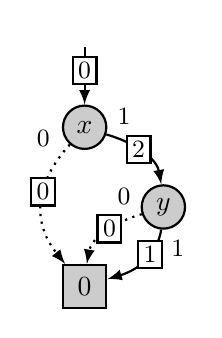
\begin{tikzpicture}[%
                costnode/.style={pos=0.6,rectangle,thick,solid,
                                inner sep=2pt,draw,fill=white,text=black,font=\small},%
                decisionnode/.style={circle,thick,minimum size=4mm,
                                inner sep=2pt,draw,fill=white!80!black,text=black,font=\normalsize},%
                xscale=2,yscale=1.35,>=latex]
        \node[] (before) at (0,2.35) {}; % incoming edge_value
        \node[decisionnode, minimum size=0.55cm] (x) at (0,1.5) {$x$};
        \node[decisionnode, minimum size=0.55cm] (y) at (0.5,0.75) {$y$};
        \node[draw,thick,fill=white!80!black,rectangle, minimum size=0.55cm]
        (after0) at (0,0) {{$0$}};
        \draw[->, thick] (before) to[bend right=0,label distance=0mm,edge
        label={},swap,pos=0.3] node[costnode,pos=0.4] {$0$} (x);
        % x =>
        \draw[->, thick, dotted] (x) to[bend right=30,label distance=0mm,edge
        label={\small{$0$}},swap,pos=0.1] node[costnode,pos=0.4] {$0$} (after0);
        \draw[->, thick] (x) to[bend left=30,label distance=0mm,edge
        label={\small{$1$}},pos=0.01] node[costnode,pos=0.4] {$2$} (y);
        % y =>
        \draw[->, thick, dotted] (y) to[bend right=30,label distance=0mm,edge
        label={\small{$0$}},swap,pos=0.01] node[costnode,pos=0.4] {$0$} (after0);
        \draw[->, thick] (y) to[bend left=30,label distance=0mm,edge
        label={\small{$1$}},pos=0.01] node[costnode,pos=0.4] {$1$} (after0);
\end{tikzpicture}

    }
  }
  \\
  \subfloat[BDD $B_{f=0}$ representing the characteristic function $\charf_S = \lnot x$ with size $|B_{f=0}| = 3$.\label{fig:bdd_0}]{
  \centering
  \makebox[0.3\textwidth][c]{
    \input{figures/background_bdd_0}
  }
  }\hfill
  \subfloat[BDD $B_{f=2}$ representing the characteristic function $\charf_S = x \land \lnot y$ with size $|B_{f=2}| = 4$.\label{fig:bdd_2}]{
  \centering
  \makebox[0.3\textwidth][c]{
    \input{figures/background_bdd_2}
  }
  }\hfill
  \subfloat[BDD $B_{f=3}$ representing the characteristic function $\charf_S = x \land y$ with size $|B_{f=3}| = 4$.\label{fig:bdd_3}]{
  \centering
  \makebox[0.3\textwidth][c]{
    
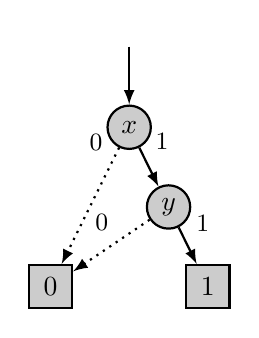
\begin{tikzpicture}[%
                costnode/.style={pos=0.6,rectangle,thick,
                                inner sep=2pt,draw,fill=white,text=black,font=\normalsize},%
                decisionnode/.style={circle,thick,minimum size=4mm,
                                inner sep=2pt,draw,fill=white!80!black,text=black,font=\normalsize},%
                xscale=2,yscale=1.35,>=latex]
        \node[] (before) at (0,2.35) {}; % incoming edge_value
        \node[decisionnode, minimum size=0.55cm] (x) at (0,1.5) {$x$};
        \node[decisionnode, minimum size=0.55cm] (y) at (0.25,0.75) {$y$};
        \node[draw,thick,fill=white!80!black,rectangle, minimum size=0.55cm]
        (after0) at (-0.5,0) {{$0$}};
        \node[draw,thick,fill=white!80!black,rectangle, minimum size=0.55cm]
        (after1) at (0.5,0) {{$1$}};
        \draw[->, thick] (before) to (x);
        % x =>
        \draw[->, thick, dotted] (x) to[bend right=0,label distance=0mm,edge
        label={\small{$0$}},swap,pos=0.1] (after0);
        \draw[->, thick] (x) to[bend left=0,label distance=0mm,edge
        label={\small{$1$}},pos=0.3] (y);
        % y =>
        \draw[->, thick, dotted] (y) to[bend right=0,label distance=0mm,edge
        label={\small{$0$}},swap,pos=0.4] (after0);
        \draw[->, thick] (y) to[bend left=0,label distance=0mm,edge
        label={\small{$1$}},pos=0.4] (after1);
\end{tikzpicture}

  }
  }\hfill
  \caption{Visualization of different decision diagrams.}
  %The ADD $A_f$ and EVBDD $E_f$ directly represent the numerical function $f = 2x + xy$. The BDDs $B_{f=z}$ represent all states for which the evaluation of the function $f$ is $z$.}
  % used to represent characteristic and numeric functions.}
  \label{fig:bdd_add}
\end{figure}

The size of a decision diagram depends strongly on the variable order, so that a good order can lead to an exponentially more compact decision diagram \autocite{edelkamp-kissmann-aaai2011}. For some functions the size of the corresponding decision diagram is exponential, independent of the underlying variable order \autocite{bryant-ieeecomp1986,edelkamp-kissmann-aaai2011}. Comparing the different types of decision diagrams, we can see that an EVBDD can be exponentially more compact than an ADD \autocite{roux-siminiceanu-nfm2010} representing additively separable functions such as $f: \{ 0,1 \}^{n+1} \to \{0, \dots, 2^{n+1}-1\}$ with $f(x_0, \dots, x_n) = \sum_{i=0}^{n} 2^i x_i$. Moreover, an ADD can be efficiently disassembled into multiple BDDs, one for each terminal node, in polynomial time and memory with respect to the ADD size by substituting terminal nodes \autocite{torralba-phd2015}. In practice, the main advantage of using BDDs over ADDs (and EVBDDs) is that decision diagram libraries such as \name{cudd} \autocite{somenzi-cudd2015} use techniques such as complement edges to store BDDs more compactly \autocite{brace-et-al-acm1990} and allow for more efficient operations \autocite{burch-et-al-tcad1994}.

\begin{example}\label{ex:dds}
  \Cref{fig:add,fig:evbdd} show the ADD $A_f$ and EVBDD $E_f$ representing the numeric function $f = 2x + xy$. 
  The function $f$ can also be represented as multiple BDDs by disassembling the ADD $A_f$ into three different BDDs, one for each terminal node. \Cref{fig:bdd_0,fig:bdd_2,fig:bdd_3} depict the BDDs $B_{f=z}$ representing all states for which the evaluation of function $f = 2x + xy$ is $z$. The variable order for all decision diagrams is $x \succ y$, i.e., x appears before y on each path.
\end{example}

From now on, 
%in the context of symbolic search,
when we refer to state sets, characteristic functions and numerical functions, we assume that they are represented as one of the corresponding decision diagrams and all logical or numerical operations are realized with the efficient and appropriate decision diagram-based operations using the \algname{apply} algorithm \autocite{bryant-ieeecomp1986,bahar-et-al-fmsd1997,lai-et-al-ieeetc1996}. If it is important which type of decision diagram we have used to represent certain functions, we will specify it explicitly.


%\section{Empirical Experiments}
%\todo{Talk shortly about symple, symk which is based on symba and fast-downward. We will use this planner in all empirical evaluations}
